\documentclass[12pt, a4paper]{article}

\usepackage[czech]{babel}
\usepackage{lmodern}
\usepackage[utf8]{inputenc}
\usepackage[T1]{fontenc}
\usepackage[pdftex]{graphicx}
\usepackage{amsmath}
\usepackage[hidelinks,unicode]{hyperref}
\usepackage{float}
\usepackage{listings}
\usepackage{tikz}
\usepackage{xcolor}
\usepackage{tabularx}
\usepackage[final]{pdfpages}


\definecolor{mauve}{rgb}{0.58,0,0.82}
\usetikzlibrary{shapes,positioning,matrix,arrows}

\newcommand{\img}[1]{(viz obr. \ref{#1})}

\definecolor{pblue}{rgb}{0.13,0.13,1}
\definecolor{pgreen}{rgb}{0,0.5,0}
\definecolor{pred}{rgb}{0.9,0,0}
\definecolor{pgrey}{rgb}{0.46,0.45,0.48}

\lstset{frame=tb,
  language=C,
  aboveskip=3mm,
  belowskip=3mm,
  showstringspaces=false,
  columns=flexible,
  basicstyle={\small\ttfamily},
  numbers=none,
  numberstyle=\tiny\color{gray},
  keywordstyle=\color{blue},
  commentstyle=\color{pgreen},
  stringstyle=\color{mauve},
  breaklines=true,
  breakatwhitespace=true,
  tabsize=3
}


\let\oldsection\section
\renewcommand\section{\clearpage\oldsection}

\begin{document}
	% this has to be placed here, after document has been created
	% \counterwithout{lstlisting}{chapter}
	\renewcommand{\lstlistingname}{Ukázka kódu}
	\renewcommand{\lstlistlistingname}{Seznam ukázek kódu}
    \begin{titlepage}

        \centering

        \vspace*{\baselineskip}
        \begin{figure}[H]
        \centering
        
\includegraphics[width=7cm]{img/fav-logo.jpg}
        \end{figure}

        \vspace*{1\baselineskip}

        \vspace{0.75\baselineskip}

        \vspace{0.5\baselineskip}
        {Semestrální práce z předmětu KIV/OS}

        {\LARGE\sc Simulace operačního systému\\}

        \vspace{4\baselineskip}

        \vspace{0.5\baselineskip}

        {\sc\Large Eliška Mourycová \\}
        \vspace{0.5\baselineskip}
        {A20N0061P}

        {\sc\Large Ondřej Drtina \\}
        \vspace{0.5\baselineskip}
        {A20N0077P}

        {\sc\Large Stanislav Král \\}
        \vspace{0.5\baselineskip}
        {A20N0091P}

        \vfill

        {\sc Západočeská univerzita v Plzni\\
        Fakulta aplikovaných věd}

    \end{titlepage}


    % TOC
    \tableofcontents
    \pagebreak

    
	\section{Zadání}
	Zadáním semestrální práce byla simulace operačního systému. Úkolem bylo navrhnout a s využitím připravené kostry simulátoru v jazyce C++ implementovat aplikaci, která bude simulovat chování operačního systému.
	
	Pro simulaci bylo potřeba navrhnout a implementovat správu procesů, vláken a otevřených souborů, souborový systém FAT s využitím přiloženého obrazu diskety, roury a přesměrování a konkrétní uživatelské příkazy a programy. %... todo co jeste
	
		\subsection{Požadované programy}
		Seznam a stručný popis požadovaných uživatelských programů je uveden zde (pro podrobnější popis jednotlivých příkazů viz podsekci \ref{subDetail}):


\begin{table}[!ht]
\centering
\begin{tabularx}{\textwidth}{r|p{11cm}}
\textbf{Příkaz} & \textbf{Význam}                                                                                                                 
\\
\hline
\texttt{echo}            & Vypíše řetězec zadaný v argumentu                                                                                                \\
\texttt{cd}              & Změní pracovní adresář aktuálního shellu                                                                                         \\
\texttt{dir}             & Vypíše položky, které se nachází v zadaném adresáři                                                                              \\
\texttt{md}              & Vytvoří nový adresář                                                                                                             \\
\texttt{rd}              & Smaže zadaný adresář
\\
\texttt{type}            & Vypíše obsah zadaného souboru                                                                                                    \\
\texttt{find}            & Vypíše počet řádek zadaného souboru                                                                                              \\
\texttt{sort}            & Seřadí jednotlivé řádky zadaného souboru                                                                                         \\
\texttt{tasklist}        & Vypíše seznam běžících procesů                                                                                                   \\
\texttt{shutdown}        & Ukončí všechny procesy                                                                                                           \\
\texttt{rgen}            & Začne vypisovat náhodně vygenerovaná čísla v plovoucí čárce                                                                      \\
\texttt{freq}            & Sestaví frekvenční tabulku bytů, kterou pak vypíše pro všechny byty s frekvencí větší než 0
\\
\texttt{shell}			 & Spustí nový shell
\\
\texttt{exit}			 & Ukončí aktuální shell
\end{tabularx}
\caption{Požadované příkazy shellu}
\label{tabCommands}
\end{table}




\section{Uživatelská příručka}
	Tato sekce popisuje ovládání simulátoru.    
    
    \subsection{Spuštění simulátoru}
Program spustíte dvojitým kliknutím na spustitelný soubor \texttt{boot.exe}, který se nachází v adresáři \texttt{compiled}. Zobrazí se terminálové okno, které je připraveno na přijímání příkazů.    

Okno zobrazuje prompt (po spuštění ve formátu \texttt{C:\textbackslash>}). V promptu se nastavuje informace o pracovním adresáři shellu.
    
    \subsection{Zadávání příkazů}
	Simulátor dokáže vykonat podporované příkazy (viz tabulku \ref{tabCommands}). Příkazy lze vykonat samostatně nebo je řadit do tzv. pipelines pomocí symbolu |, popř. přesměrovat obsah souboru na vstup prvního procesu pomocí < a výstup posledního procesu do souboru pomocí >.
	Např.:    
	\begin{lstlisting}[language=C, caption={Příklad pipeline},captionpos=b]
    C:\> p1 | p2 | p3 > out.txt < in.txt
    \end{lstlisting}
    
    Uživatel je informován o případné nemožnosti vykonání příkazu.
    
    
    \subsection{Ukončení simulace}
    Simulaci je možné ukončit příkazem \texttt{shutdown}. Pokud je spuštěný pouze jeden shell, příkaz \texttt{exit} také ukončí simulaci.




    \section{Kernel}

    Kernel je část operačního systému, která provádí inicializaci hardwaru, zajišťuje správu prostředků a umožňuje vytvářet programy či vlákna. Uživatelskému prostoru nabízí své služby pomocí tzv. systémových volání. V této semestrální práci lze kernel rozdělit do následujících částí: 
\begin{itemize}
    \item správa procesů/vláken
    \item správa otevřených souborů
    \item souborový systém FAT12
\end{itemize}

\subsection{Správa procesů a vláken}
Tuto část kernelu lze považovat za nejdůležitější, jelikož bez její přítomnosti by nebylo možné spouštět žádné programy. Stará se o vytváření procesů a jejich správu, kdy lze procesy synchronizovat a nastavovat jejich návratové hodnoty. Simulace vláken a procesů je realizována pomocí konstrukcí pro vytváření vláken ze standardní knihovny \texttt{thread}. Většina kódu této části se nachází v souboru \texttt{/kernel/process.cpp}.

Pro použití služeb této části kernelu z uživatelského prostoru slouží následující systémová volání ze skupiny \texttt{Process}.

\begin{itemize}
    \item \texttt{Clone},
    \item \texttt{Wait\_For},
    \item \texttt{Read\_Exit\_Code},
    \item \texttt{Exit},
    \item \texttt{Register\_Signal\_Handler}
\end{itemize}

\subsubsection{Vytvoření nového vlákna}

Nativní identifikátory vytvořených vláken jsou mapovány na typ \texttt{kiv\_os::THandle}, který se dále používá v rámci kernelu jako interní identifikátor vláken.

Při zpracování požadavku na vytvoření nového vlákna se ze vstupních registrů načtou potřebné argumenty, a zavolá se funkce \texttt{run\_in\_a\_thread}, která přebírá argument obsahující vstupní bod části kódu, jež se má spustit v novém vlákně. Tato funkce vytvoří nové \texttt{std::thread} vlákno, kterému jako vstupní funkci nastaví funkci \texttt{thread\_entrypoint} přebírající skrz argumenty vstupní bod kódu ke spuštění. Uvnitř spuštěného vlákna se před vykonáváním kódu dále čeká, dokud kernel nepřidá toto vlákno do tabulky všech vláken. Čekání je realizováno pomocí semaforu, a teprve po jeho notifikaci se začne vykonávat požadovaný kód. 

Při vytváření nového vlákna se navíc dohledává, jaké vlákno či proces nové vlákno vytváří. Tato informace se později využívá např. při změně pracovního adresáře procesu.

\subsubsection{Synchronizace vláken}
Jádro umožňuje synchronizaci vytvořených vláken pomocí systémového volání \texttt{Wait\_For}. Obsluha tohoto volání je realizována pomocí funkce \texttt{wait\_for}, která přebírá pole obsahující identifikátory vláken, na která se má čekat. Synchronizace je realizována pomocí semaforů, kdy ke každému běžícímu vláknu je veden seznam semaforů, které se mají při skončení vlákna notifikovat. Jeden semafor může tedy být přiřazen k více než jednomu vláknu. 

Na začátku obsluhy je k daným vláknům přiřazen nově vytvořený semafor, a zahájí se čekání na notifikaci tohoto semaforu. V moment, kdy je daný semafor notifikován, je vlákno čekající na semafor probuzeno, a tento semafor je odebrán ze všech ostatních seznamů, kde se vyskytuje. Spolu s notifikací semaforu je čekajícímu vláknu předána i informace o tom, jaké vlákno semafor probudilo. 

\begin{figure}[!ht]
\centering
{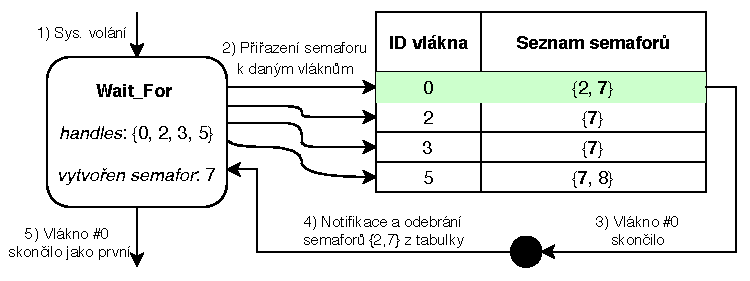
\includegraphics[width=14.5cm]{pdf/wait_for.pdf}}
\caption{Zjednodušený diagram obsluhy sys. volání \texttt{Wait\_For}}
\label{fig:screen-transition-diagram}
\end{figure}

\subsubsection{Vytváření procesů}
Vytváření procesů je principiálně stejné jako vytváření vláken a používá se stejných funkcí jako při vytváření nového vlákna. Hlavním rozdílem je to, že až v jádře se převádí název programu na vstupní bod programu, který se předává funkci \texttt{run\_in\_a\_thread}. Před zahájením vykonávání kódu programu je po vytvoření nového vlákna dle jeho identifikátoru přidán nový záznam do tabulky všech procesů. Dále také nový proces dědí pracovní adresář od procesu, kterým byl vytvořen.

Tabulka procesů, která je v kódu implementována třídou\\ \texttt{Process\_Control\_Block}, obsahuje následující sloupce:
\begin{itemize}
    \item \texttt{kiv\_os::THandle handle} - identifikátor (\textbf{PID}\footnote{process identifier}) procesu,
    \item \texttt{kiv\_os::THandle std\_in} - identifikátor standardního vstupu procesu,
    \item \texttt{kiv\_os::THandle std\_out} - identifikátor standardního výstupu procesu,
    \item \texttt{char *program\_name} - název programu, který proces vykonává,
    \item \texttt{std::filesystem::path working\_directory} - aktuální pracovní adresář procesu,
    \item \texttt{kiv\_os::NOS\_Error exit\_code} - návratová hodnota procesu programu, který proces vykonává,
    \item \texttt{Process\_Status status} - stav procesu, který může nabývat hodnot \texttt{Ready}, \texttt{Running}, \texttt{Zombie}
\end{itemize}

Předtím, než proces začne vykonávat kód programu, setrvává ve stavu \texttt{Process\_Status::Ready}. Během vykonávání programu setrvává ve stavu \texttt{Process\_Status::Running}. Pokud proces již dokončil vykonávání kódu programu, potom setrvává ve stavu \texttt{Process\_Status::Zombie}, dokud si jiný proces nepřečte jeho návratovou hodnotu. 

\subsubsection{Nastavení návratové hodnoty procesu}
Všem procesům je při jejich vytvoření nastavena výchozí návratová hodnota \texttt{kiv\_os::NOS\_Error::Success}. V případě, že nějaký program chce tuto hodnotu nastavit ručně, tak má možnost použít systémové volání \texttt{Exit}, a v registrech nastavit požadovanou návratovou hodnotu.

\subsubsection{Přečtení návratové hodnoty procesu}
Přečtení návratové hodnoty procesu z uživatelského prostoru je možné pomocí systémového volání \texttt{Read\_Exit\_Code}, kdy je před voláním nutné nastavit do registrů identifikátor procesu, jehož návratovou hodnotu chceme přečíst.

Toto volání je implementováno tak, že se nejdřív zkontroluje, jestli daný proces již skončil a setrvává ve stavu \texttt{Process\_Status::Zombie}. Pokud ano, tak se jednoduše z tabulky získá jeho návratová hodnota. V případě, že proces ještě neskončil, tak v tomto stavu nesetrvává, a tudíž nelze v tuto chvíli přečíst jeho návratovou hodnotu, protože by se ještě mohla změnit. Obsluha systémového volání \texttt{Read\_Exit\_Code} tedy zavolá funkci \texttt{wait\_for} a počká, dokud daný proces neskončí. Poté přečte a vrátí jeho návratovou hodnotu.

 Na konci tohoto volání po úspěšném přečtení návratové hodnoty je z tabulky procesů daný proces, jehož návratovou hodnotu jsme přečetli, odebrán.

\subsubsection{Nastavení obsluhy systémového signálu aktuálního procesu}
Aby každý proces mohl nastavit vlastní obsluhu libovolného systémového signálu, jádro poskytuje možnost volat systémové volání\\ \texttt{Register\_Signal\_Handler}.

Kontrakt definovaný v \texttt{/api/api.h} umožňuje použít jednu obsluhu víckrát a nastavit ji pro více signálů. Implementace tohoto kontraktu je realizována tak, že každý proces má vlastní tabulku, kde klíčem je signál a hodnotou je adresa obsluhy daného signálu.

\begin{figure}[!ht]
\centering
{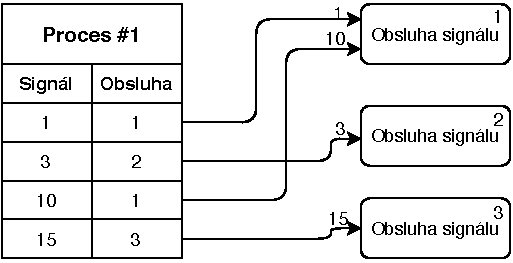
\includegraphics[width=11.5cm]{pdf/register_signal_handler.pdf}}
\caption{Vizualizace tabulky obsluh systémových signálů jednoho procesu}
\label{fig:screen-transition-diagram}
\end{figure}

Při rozeslání signálu jádrem se dle tabulky obsluh každého procesu dohledává, která obsluha se má zavolat. Pokud některý z procesů nemá nastavenou vlastní obsluhu daného signálu, zavolá se výchozí obsluha signálu definovaná kernelem.

\subsection{Implementace rour}
Aby bylo možné přesměrovávat výstup jednoho procesu do vstupu jiného, je třeba, aby jádro umožňovalo vytvářet roury, které mají vstup, výstup a paměťový buffer.

Implementace rour představuje rozšíření řešení problému \textit{producent a konzument}. Třída, jejíž instance představují samotné roury, je definována v souborech \texttt{kernel/pipe.h} a \texttt{kernel/pipe.cpp}. V konstruktoru přijímá velikost bufferu, podle které dále inicializuje dva semafory. Volajícímu poskytuje následující metody:

\begin{itemize}

    \item \texttt{std::vector<char> Pipe::Read(size\_t read, bool \&empty)} - tato metoda, která představuje konzumenta a slouží ke čtení požadovaného množství dat z bufferu, přijímá v druhém parametru referenci na booleanskou hodnotu, kterou nastaví na \texttt{true}, pokud byl přečten celý dostupný obsah bufferu a vstup roury byl zavřen. V takový moment již není co číst a nelze očekávat, že do bufferu bude cokoliv zapsáno, protože vstup byl již zavřen.

    \item \texttt{size\_t Pipe::Write(std::vector<char> data)} - tato metoda představující producenta slouží k zapisování předaných dat do bufferu a vrací počet zapsaných bytů. Pokud byl v průběhu zápisu zavřen výstup nebo vstup roury, zapisování je přerušeno.

    \item \texttt{void Pipe::Close\_Out()} - slouží k zavření výstupu, kdy po zavření notifikuje semafory pro zápis i čtení, aby bylo možné oznámit vláknům čekajícím na zápis nebo čtení událost zavření výstupu.

    \item \texttt{void Pipe::Close\_In()} - slouží k zavření vstupu, kdy nejdřív zapíše znak \texttt{EOT} a až poté vstup zavře. 

\end{itemize}

Pro vytvoření rour z uživatelského prostředí slouží systémové volání \texttt{Create\_Pipe}, které vytvoří nový objekt roury, dvakrát jej vloží do tabulky souborů (jedno pro zápis a jednou pro čtení) a vygenerované identifikátory (indexy do souoborové tabulky) zapíše do registrů.


\subsection{Tabulka souborů}
K uložení informací o aktuálně otevřených souborech slouží tzv. tabulka souborů. Taková tabulka v sobě obsahuje seznam všech aktuálně otevřených souborů, kdy každý záznam v tabulce představuje jedno otevření souboru a může obsahovat informaci o způsobu, jakým byl otevřen (např. atributy \texttt{kiv\_os::NFile\_Attribtues}). Tento záznam také obsahuje odkaz na instanci implementace abstraktní třídy \texttt{Generic\_File}, která definuje, jak se z daného souboru čte. V této semestrální práci jsou implementovány následující typy souborů:

\begin{itemize}

    \item soubor souborového systému -- implementován ve třídě \texttt{Filesystem\_File} a v konstruktoru přebírá odkaz na rozhraní souborového systému, kterým může být souborový systém FAT nebo \texttt{procfs}, který slouží ke čtení z tabulky procesů.

    \item soubor vstupu roury -- implementován ve třídě \texttt{Pipe\_In\_File} a v konstruktoru přebírá odkaz na instanci roury. Tento soubor podporuje pouze zápis, a zapisuje do roury.

    \item soubor výstupu roury -- implementován ve třídě \texttt{Pipe\_Out\_File} a v konstruktoru přebírá odkaz na instanci roury. Tento soubor podporuje pouze čtení, a čte z roury.

    \item soubor klávesnice -- implementován ve třídě \texttt{Keyboard\_File} a umožňuje číst z klávesnice, potažmo z konzole. Umožňuje i zápis, který zapisuje do virtuálního bufferu klávesnice.

    \item soubor textového výstupu -- implementován ve třídě \texttt{Tty\_File} a umožňuje zapisovat do konzole.

\end{itemize}

Tato tabulka je implementovaná jako třída obalující \texttt{std::map<kiv\_os::THandle, std::unique\_ptr<Generic\_File>>}. Otevřením nového souboru vznikne v této tabulce nový záznam, a při zavření je z tabulky odebrán.

\begin{table}[ht]
\centering
\begin{tabular}{|l|l|}
\hline
\textbf{Identifikátor} & \textbf{Obecný souborový objekt} \\ \hline
1                      & \texttt{Keyboard\_File}                   \\ \hline
2                      & \texttt{Tty\_File}                        \\ \hline
3                      & \texttt{Pipe\_In\_File}                   \\ \hline
4                      & \texttt{Pipe\_Out\_File}                  \\ \hline
5                      & \texttt{Fs\_File}                         \\ \hline
\end{tabular}
\caption{Ukázka tabulky obecných souborových objektů}
\end{table}

Díky této implementaci je tedy zápis a čtení do souborů jednoduchý, protože logika implementace je volajícímu schovaná -- stačí pouze znát identifikátor požadovaného souboru.

\subsubsection{Operace nad soubory}
Nad soubory lze provádět různé operace pomocí následujících systémových volání:

\begin{itemize}
    \item \texttt{Read\_File} -- vyhledá v tabulce souborů daný soubor a provede čtení,
    \item \texttt{Write\_File} -- vyhledá v tabulce souborů daný soubor a provede zápis,
    \item \texttt{Close\_File} -- vyhledá v tabulce souborů daný soubor, zavře ho a odstraní ho ze souborové tabulky,
    \item \texttt{Seek} -- vyhledá v tabulce souborů daný soubor, a dle zadaných parametrů provede jeho zvětšení nebo změnu aktuální pozice kurzoru,
    \item \texttt{Get\_File\_Attribute} -- vyhledá v tabulce souborů daný soubor, a vrátí jeho atributy,
    \item \texttt{Seek\_File\_Attribute} -- vyhledá v tabulce souborů daný soubor, a změní jeho atributy, 
    \item \texttt{Delete\_File} -- vyhledá dle specifikované cesty v připojených souborvých systémech soubor, a pokud existuje, tak se ho pokusí smazat.
\end{itemize}

\subsection{Obecné rozhraní souborového systému}
Každý souborový systém, který by má být podporován jádrem, musí implementovat rozhraní virtuálního souborového systému. Toto rozhraní je definováno v abstraktní třídě \texttt{VFS}. Definuje hlavičky metod pro následující operace:
\begin{itemize}
    \item vytvoření nové složky
    \item odstranění složky
    \item přečtení obsahu složky
    \item otevření souboru (buď již existujícího nebo nově vytvořeného)
    \item zápis
    \item čtení
    \item odstranění souboru
    \item ověření existence souboru ve specifikované složce 
    \item nastavení a získání atributů souboru 
\end{itemize}

Tato třída implementuje metodu \texttt{generate\_dir\_vector}, která v parametrech přebírá seznam položek složky (seznam struktur \texttt{kiv\_os::TDir\_Entry}) a převede je na seznam znaků (\texttt{char}), aby bylo možné tento seznam přečíst z uživatelského prostoru.

Tento způsob definice rozhraní souborového systému umožňuje flexibilní přidávání dalších podporovaných systémů, kdy stačí pouze implementovat dané rozhraní a definovat, na jaké cestě se nachází kořen souborového systému. 

\subsubsection{Ověření existence souboru}
Z uživatelského prostoru může přijít požadavek na otevření souboru, jehož adresa může být specifikována buď jako relativní nebo absolutní. Pro jednodušší práci s adresami se používá typ \texttt{std::filesystem::path} ze standardní knihovny. Pokud byla specifikována relativně, tak se vždy na začátek této adresy ještě přidá aktuální pracovní adresář, a začne ověřování existence jednotlivých komponent cesty.

\noindent Ověření existence cesty \texttt{A} používá následující algoritmus:

\begin{enumerate}
    \item načti komponentu adresy a přidej jí do \texttt{P}
    \item zjisti, jaký souborový systém \texttt{S} se na \texttt{P} používá, 
    \item ověř existenci souboru na cestě \texttt{P} pomocí \texttt{S}
    \item pokud na \texttt{P} v \texttt{S} soubor neexistuje -- \textbf{cesta je neplatná}
    \item pokud existuje a cesta obsahuje další komponentu, běž na \textbf{1.}
    \item pokud existuje a cesta již neobsahuje další komponentu, \texttt{P} \textbf{ukazuje na platný soubor} v \texttt{S}
\end{enumerate}

Při změně aktuálně používaného souborového systému se do ADT struktury zásobník přidá na vrchol dosud používaný souborový systém. V každém souborovém systému se počítá počet zanoření. Zpracování komponenty \texttt{..} snižuje počet zanoření v stromové struktuře složek. Pokud počet zanoření dosáhne nulové hodnoty, tak se ze zásobníku vyjme poslední používaný souborový systém. Využití zásobníku snižuje počet vyhledávání kořenů souborových systémů. 

\subsection{Pracovní adresář} \label{wd}
Pomocí systémových volání \texttt{Set\_Working\_Dir} a \texttt{Get\_Working\_Dir} se mění a získává pracovní adresář aktuálního procesu (tj. toho, který inicializoval systémové volání). Při změně adresáře se pomocí algoritmu ukázaném v podkapitole \ref{wd} kontroluje existence adresáře nacházajícího se na zadané cestě. Dále se také kontroluje, zdali cesta opravdu ukazuje na adresář, a ne například na obyčejný soubor.

\subsection{Souborový systém \texttt{procfs}}
Aby bylo možné nechat z uživatelského prostoru vypsat obsah tabulky procesů a zobrazit tak seznam aktuálně běžících procesů, je třeba, aby v kernelu byl implementován vlastní souborový systém, který bude číst z této tabulky, a pomocí kombinace virtuálních souborů a adresáře tak zpřístupňovat seznam procesů.

V této semestrální práci se na adrese \texttt{C:\textbackslash procfs} nachází adresář, jehož položky představují položky tabulky procesů a jsou pojmenovány identifikátory procesů. Při čtení položek z tohoto adresáře jsou položky tabulky procesů převedeny na strukturu \texttt{PCB\_Entry} a uloženy v paměťovém bufferu. Dle parametrů předaných při čtení je volajícímu vrácen kus paměťového bufferu.

Jelikož v souboru \texttt{api.h} není definována struktura položky tabulky procesů, tak by uživatelský prostor nevěděl, jak obsah souborů v adresáři \texttt{procfs} interpretovat. Z tohoto důvodu byla po dohodě s vyučujícím do kernelu i uživatelského prostoru přidána struktura \texttt{PCB\_Entry}, kterou kernel vrací při čtení z adresáře \texttt{procfs}, a tak uživatelský prostor ví, jak obsah souborů interpretovat.

\subsubsection{Alternativní řešení}
Sdílení struktury mezi uživatelským prostorem a kernelem lze předejít tak, že by položky v adresáří \texttt{procfs} představovaly adresáře, které by se jmenovaly dle identifikátorů běžících procesů. V těchto adresářích by se dále nacházely soubory, kdy každý soubor by obsahoval jeden atribut daného procesu.


\subsection{Implementace souborového systému \texttt{FAT12}}
Program umožňuje vytváření souborů a složek, přičemž k jejichž uchování je využíván dodaný obraz diskety pracující se souborovým systémem \texttt{FAT12}. Funkce, jež implementují uvedený souborový systém, jsou definovány v souborech \texttt{kernel/fat\_fs.h} a \texttt{kernel/fat\_fs\_utils.h}.

\subsubsection{Definice v \texttt{kernel/fat\_fs.h}}
Obsahuje definici veškerých funkcí, které jsou volány vyššími vrstvami OS ve spojitosti s prací se souborovým systémem \texttt{FAT12}. Některé z funkcí, jež jsou v souboru uvedeny, ve svém těle volají funkce definované v souboru \texttt{kernel/fat\_fs\_utils.h}.

Třída \texttt{Fat\_Fs} dědí od abstraktní třídy \texttt{VFS} a obsahuje funkce umožňující zápis, respektive čtení souboru. Rovněž jsou obsaženy funkce, které umožňují vyšším vrstvám OS vytváření a mazání složek. Obsažena je i funkce ověřující existenci souborů a složek.

\subsubsection{Definice v \texttt{kernel/fat\_fs\_utils.h}}
Obsahuje podpůrné funkce souborového systému \texttt{FAT12}, jež nejsou přímo volány vyššími vrstvami OS, ale jsou využívány v rámci třídy \texttt{Fat\_Fs}. Jsou zde obsaženy funkce usnadňující práci se souborovým systémem. Příklady obsažených funkcí:
\begin{itemize}
    \item \texttt{int allocate\_new\_cluster()} - alokace nového clusteru (souboru / složky)
    \item \texttt{std::vector<int> retrieve\_sectors\_nums\_fs} - získání seznamu sektorů daného souboru či složky
    \item \texttt{bool check\_file\_name\_validity()} - zjištění platnosti názvu souboru ve \texttt{FAT12}.
\end{itemize}

\subsubsection{Problémy spojené s implementací}
Při implementaci souborového systému byl pro nás problémem zejména fakt, že ve \texttt{FAT12} tabulce, jež obsahuje informace o stavu clusterů, je jedna hodnota reprezentována 12 bity. Při editaci hodnot v tabulce bylo tedy třeba načíst vždy dva bajty (resp. 16 bitů) a upravit jen odpovídající část dat.

\section{User space}
	User space je část operačního systému, která pomocí systémových volání žádá kernel o služby pro obsluhu uživatelských programů. Tato logika je použita i v naší práci. Funkcionalita uživatelských programů (jejich kód, spouštění, apod.) je implementovaná v projektu \texttt{user}. Jejich spouštění a případná orchestrace do pipeline je řešena v \texttt{shell.cpp}.
	
	
	\subsection{Podrobný popis podporovaných příkazů} \label{subDetail}
	Zde je podrobnější popis podporovaných příkazů. Implementace funkcionality se nachází v příslušných \texttt{.cpp} zdrojových souborech (tj. \texttt{nazev\_prikazu.cpp}).    
    
    \subsubsection*{\texttt{echo}}
    \texttt{echo} jako argument očekává řetězec, který má vypsat na standardní výstup. Pokud se v řetězci nachází 'speciální' znaky (tj. znak | nebo < nebo >), je potřeba řetězec uzavřít do uvozovek (`` ''), pokud výstup programu echo chceme přesměrovat na vstup jiného programu nebo do souboru.
    Příklad:
    \begin{lstlisting}[language=C, caption={Ukázka chování programu echo},captionpos=b]
    > echo "hello" | freq
      0xa : 1
	   0x65 : 1
      0x68 : 1
      0x6c : 2
      0x6f : 1 /* vystup programu freq */
    > echo hello | freq
      hello | freq /* vystup programu echo */
    \end{lstlisting}
    
    Pokud je argument příkazu \texttt{echo} řetězec \texttt{on} nebo \texttt{off}, \texttt{echo} se nevykoná jako externí program, pouze skryje prompt aktuálního shellu.
    
    \subsubsection*{\texttt{cd}}
    \texttt{cd} změní pracovní adresář aktuálního shellu. Jako argument očekává cestu (relativní nebo absolutní) k novému adresáři, který má shellu nastavit jako pracovní. Pokud argument není zadaný, pracovní adresář se nemění.
    
    \texttt{cd} se nevykonává jako externí příkaz, pouze nastaví pracovní adresář aktuálního shellu.
    
    \subsubsection*{\texttt{dir}}
    \texttt{dir} na standardní výstup vypíše položky uložené v adresáři. Cesta k požadovanému adresáři se zadává jako argument příkazu. Pokud argument není zadaný, vypíše se obsah pracovního adresáře.
    
    \subsubsection*{\texttt{md}}
    \texttt{md} vytvoří nový adresář. Cesta k novému adresáři se zadává jako argument příkazu.
    
    \subsubsection*{\texttt{rd}}
    \texttt{rd} smaže adresář zadaný v argumentu.
    
    \subsubsection*{\texttt{type}}
    \texttt{type} na standardní výstup vypíše obsah zadaného souboru. Cesta k požadovanému souboru se zadává jako argument příkazu. Pokud argument není zadaný, \texttt{type} začne číst ze standardního vstupu, dokud nepřečte znak \texttt{EOT}.
    
    \subsubsection*{\texttt{find}}
    \texttt{find} na standardní výstup vypíše počet řádek zadaného souboru. Tento příkaz se zadává ve formátu \texttt{find /v /c "{}"{} file.txt}, kde \texttt{file.txt} je cesta k požadovanému souboru. Pokud cesta k souboru není zadaná, \texttt{type} začne číst ze standardního vstupu, dokud nepřečte znak \texttt{EOT}.
    
    \subsubsection*{\texttt{sort}}
    \texttt{sort} na standardní výstup vypíše abecedně seřazené řádky zadaného souboru. Pokud cesta k souboru není zadaná, \texttt{sort} začne číst ze standardního vstupu, dokud nepřečte znak \texttt{EOT}.
    
    \subsubsection*{\texttt{tasklist}}
    \texttt{tasklist} na standardní výstup vypíše tabulku procesů s informacemi o procesech, které mají v PCB záznam. 
    \\
    \\
	\texttt{tasklist} získá informace z adresáře \texttt{/procfs}. V tomto adresáři se nachází několik položek s názvy \texttt{/procfs/pid}, kde \texttt{pid} je PID procesu, který má záznam v PCB. Mezi jádrem a uživatelským prostorem se nachází sdílená struktura \texttt{PCB\_Entry}. Každý ze souborů \texttt{/procfs/pid} obsahuje jednu strukturu \texttt{PCB\_Entry}, \texttt{tasklist} tedy z každého souboru přečte velikost \texttt{PCB\_Entry} bajtů a výsledek přetypuje na \texttt{PCB\_Entry}. Získané informace naformátuje do výsledné tabulky.
    
    
    \subsubsection*{\texttt{shutdown}}
    \texttt{shutdown} ukončí všechny běžící procesy, tj. vč. všech spuštěných shellů.
    
    \subsubsection*{\texttt{rgen}}
    \texttt{rgen} začne na standardní výstup vypisovat náhodné byty. Ne však byty s hodnotou 0x04, tj. znak \texttt{EOT}.
    
    \subsubsection*{\texttt{freq}}
    \texttt{freq} začne číst ze standardního vstupu, dokud nepřečte znak \texttt{EOT}. Poté na standardní výstup vypíše frekvenční tabulku bytů pro všechny byty s frekvencí větší než 0.
    
    \subsubsection*{\texttt{shell}}
    Příkaz \texttt{shell} spustí nový shell.
    
    \subsubsection*{\texttt{exit}}
    Příkaz \texttt{exit} ukončí aktuální shell.
	
	
	\subsection{Spouštění uživatelských programů}
	Při zadání vstupního řetězce uživatelem je řetězec rozdělen na jméno programu a argumenty (popř. jména, pokud vstup obsahuje symbol roury nebo přesměrování).	
	
	
	Po zadání příkazu se pokusíme příslušný program spustit pomocí systémového volání \texttt{kiv\_os\_rtl::Clone\_Process}. Jméno programu se nekontroluje, kontroluje se pouze návratová hodnota systémového volání. Pokud vše proběhlo v pořádku, v novém vlákně je spuštěn daný proces.
	
	Po skončení procesu je přečten jeho návratový kód pomocí systémového volání \texttt{kiv\_os\_rtl::Read\_Exit\_Code}.
	
	\subsubsection{Orchestrace pipeline} 
	Pokud je potřeba přesměrovat výstup procesu na vstup jiného pomocí rour, je potřeba spustit několik procesů po sobě. 

	Nejdříve je vytvořeno dostatečné množství rour pomocí systémového volání \texttt{kiv\_os\_rtl::Create\_Pipe}. \texttt{Handles} vstupů a výstupů jednotlivých rour jsou uloženy.	
	
	Procesy jsou spouštěny od posledního k prvnímu, tj. pokud vstup vypadá např. takto:
	
	\texttt{C:\textbackslash> p1 | p2 | p3},\\
	potom prvním spuštěným procesem bude \texttt{p3} a posledním \texttt{p1}.
	
	Procesy jsou spouštěny tímto způsobem z toho důvodu, že pokud uživatel zadá neplatný příkaz, potom je potřeba všechny (již spuštěné) procesy ukončit. Pokud by první proces v pipeline byl spuštěn a potom bylo nutné jej předčasně ukončit, jedinou možností by bylo poslat na jeho vstup znak \texttt{EOT}, protože standardní vstup shellu nechceme zavírat. To s sebou ale nese komplikace. V případě spouštění od posledního k prvnímu taková situace nemůže nastat (pokud by první zadaný příkaz byl neplatný, nebude vůbec spuštěn).
	
	Při předčasném ukončování procesů jsou zavřeny \texttt{Handles} vstupů a výstupů všech rour a otevřených souborů a nakonec jsou přečteny \texttt{ExitCodes} procesů.
	\\
	\\
	Pokud jsou všechny zadané příkazy platné, jsou také všechny příslušné procesy spuštěny. Poté se začne čekat na skončení jednoho z procesů pomocí systémového volání \texttt{kiv\_os\_rtl::Wait\_For}. Jakmile jeden z procesů skončí, přečte se jeho \texttt{ExitCode} a zavře se jeho vstup a výstup (pokud se jedná o roury, nebo soubory). Toto probíhá, dokud neskončí všechny takto spuštěné procesy.





\section{Závěr}	

Zadáním semestrální práce byla simulace operačního systému. Zadání bylo z velké části splněno.

\subsection{Rozdělení práce a bodů}

Rozdělení práce mezi členy týmu vypadalo zhruba následovně (rozdělení není striktní, práce členů se v mnoha případech překrývala):

\begin{itemize}
	\item Stanislav Král (1/3 bodů)\\
		- implementace systémových volání, rour, PCB, VFS, práce v kernelu
	\item Eliška Mourycová (1/3 bodů) \\
		- práce na programech v uživatelském prostoru (parsování, implementace), orchestrace pipelines
	\item Ondřej Drtina (1/3 bodů) \\
		- práce na FS FAT s využitím přiloženého obrazu diskety, implementace VFS rozhraní
\end{itemize}

\subsection{Zhodnocení dosažených výsledků}
Přes veškerou snahu jsme bohužel nebyli schopni včas implementovat souborový systém FAT. Část jeho nutné funkcionality je implementovaná a funkční, ale nelze ho zatím integrovat do celého projektu. Avšak projekt by měl být řádně připraven na pouhé dodání implementace rozhraní VFS souborovým systémem FAT, aby mohl plně fungovat.

Máme důvěru v robustnost a správnost implementace zbytku částí projektu.

\end{document}    
